\section{Data reduction}

\begin{frame}{Data Reduction (I): Dimensionality Reduction}
	\begin{itemize}
		\item \textbf{Curse of dimensionality:}
		\begin{itemize}
			\item When dimensionality increases data becomes increasingly 
			sparse.
			\item Density and distance between points, which are critical to 
			clustering and outlier analysis become less meaningful.
			\item The possible combinations of subspaces will grow 
			exponentially.
		\end{itemize}
		\item \textbf{Dimensionality reduction:}
		\begin{itemize}
			\item Avoid the curse of dimensionality.
			\item Help eliminate irrelevant features and reduce noise.
			\item Reduce time and space required in data mining.
			\item Allow easier visualization.
		\end{itemize}
		\item \textbf{Dimensionality-reduction techniques:}
		\begin{itemize}
			\item Wavelet transforms.
			\item Principal component analysis.
			\item Supervised and nonlinear techniques (e.g. feature selection).
		\end{itemize}
	\end{itemize}
\end{frame}

\begin{frame}{Data Reduction Strategies}
	\begin{itemize}
		\item Obtain a reduced representation of the data set that is much 
		smaller in volume but yet produces the same (or almost the same)  
		results.
		\item \textbf{Why data reduction?}\\
		\begin{itemize}
			\item A database/data warehouse may store terabytes of data.
			\item Complex data analysis may take a very long time to run on the 
			complete data set.
		\end{itemize}
		\item \textbf{Data reduction strategies:}
		\begin{itemize}
			\item Dimensionality reduction, i.e. remove unimportant attributes.
			\begin{itemize}
				\item Wavelet transforms.
				\item Principal component analysis.
				\item Attribute subset selection or attribute creation.
			\end{itemize}
			\item Numerosity reduction:
			\begin{itemize}
				\item Regression and log-linear models.
				\item Histograms, clustering and sampling.
				\item Data cube aggregation.
			\end{itemize}
			\item Data compression.
		\end{itemize}
	\end{itemize}
\end{frame}

\begin{frame}{Mapping Data to a New Space}
	\begin{itemize}
		\item \textbf{Fourier transform}.
		\item \textbf{Wavelet transform.}
		
		\begin{figure}
			\centering
			\begin{minipage}[b]{0.30\textwidth}
				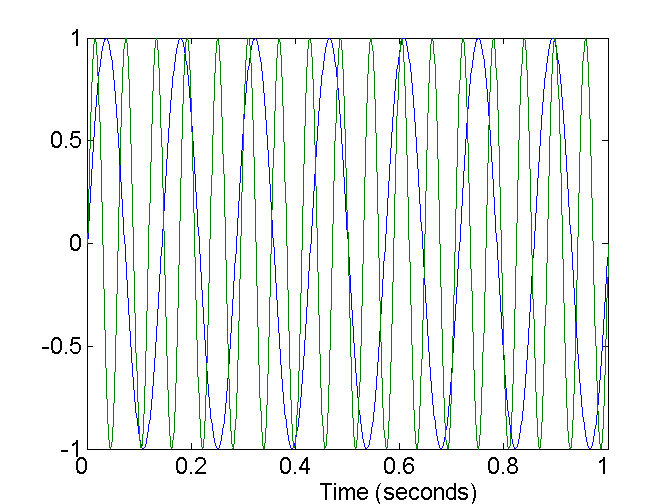
\includegraphics[width=5cm]{img/twosinewaves.png}
				\caption{Two sine waves.}
			\end{minipage}\hfill
			\begin{minipage}[b]{0.30\textwidth}
				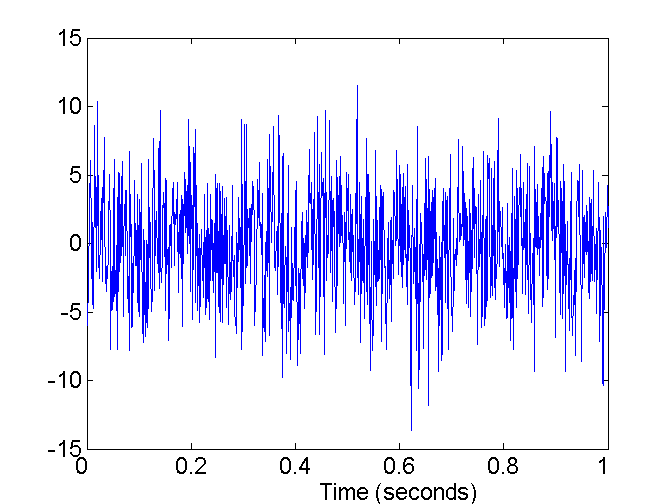
\includegraphics[width=5cm]{img/twosinewaveswithnoise.png}
				\caption{Two sine waves with noise.}
			\end{minipage}\hfill
			\begin{minipage}[b]{0.30\textwidth}
				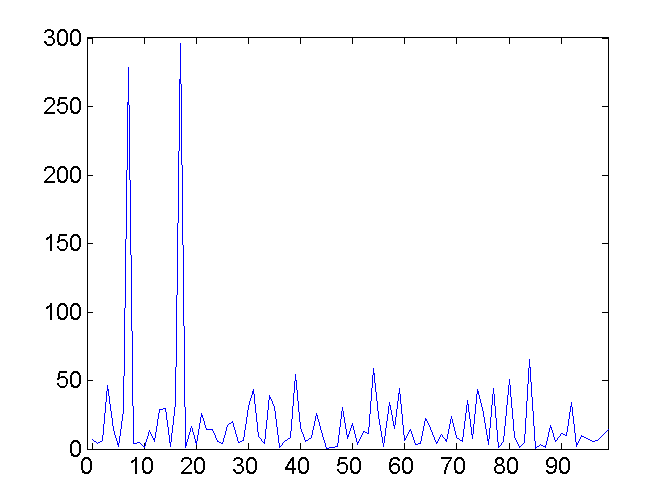
\includegraphics[width=5cm]{img/frequencies.png}
				\caption{Frequencies.}
			\end{minipage}
		\end{figure}
	\end{itemize}
\end{frame}

\begin{frame}{What is Wavelet Transform?}
	\begin{minipage}[b]{0.55\textwidth}
		\begin{itemize}
			\item \textbf{Decomposes a signal into different frequency 
			subbands.}\\
			Applicable to $n$-dimensional signals.
			\item Data transformed to preserve relative distance between 
			objects at different levels of resolution.
			\item Allow natural clusters to become more distinguishable.
			\item Used for image compression.
		\end{itemize}
	\end{minipage}\hspace{1cm}
	\begin{minipage}[b]{0.30\textwidth}
		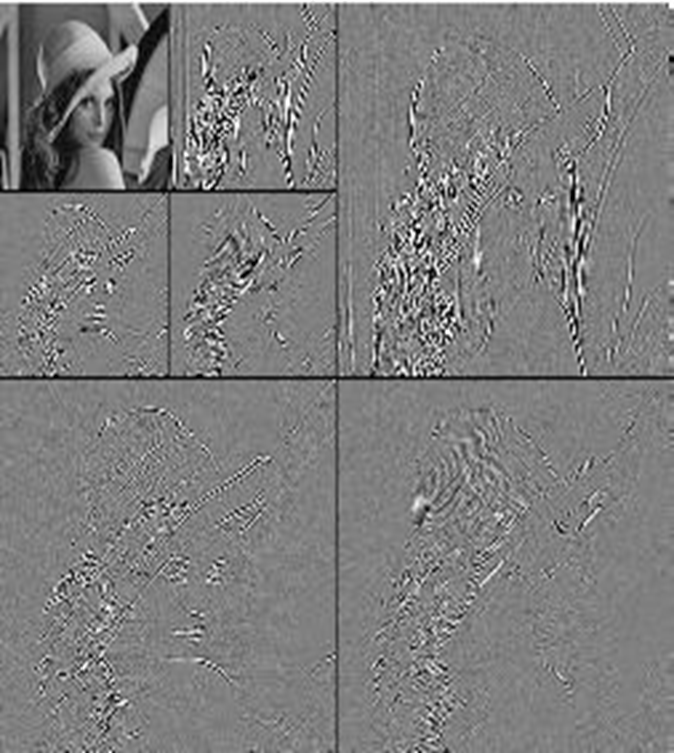
\includegraphics[width=5cm]{img/wavelettransform.png}
	\end{minipage}
\end{frame}

\begin{frame}{Wavelet Transform}
	\begin{itemize}
		\item \textbf{Discrete wavelet transform:}\\
		Transforms a vector $X$ into a different vector $X'$ of wavelet 
		coefficients with the same length.
		\item \textbf{Compressed approximation:}\\
		Store only a small fraction of the strongest of the wavelet 
		coefficients.
		\item \textbf{Similar to discrete fourier transform, but better lossy 
		compression, localized in space.}
		\item \textbf{Method:}
		\begin{itemize}
			\item The length of the vector must be an integer power of $2$ 
			(padding with $0$'s if necessary).
			\item Each transform has two functions: smoothing and difference.
			\item Applied to pairs of data, resulting in two sets of data with 
			half the length.
			\item The two functions are applied recursively until reaching the 
			desired length.
		\end{itemize}
	\end{itemize}
\end{frame}

\begin{frame}{Wavelet Decomposition}
	\begin{itemize}
		\item \textbf{Example:}
		\begin{align}
			X  & = (2,2,0,2,3,5,4,4), \text{can be transformed to} \\
			X' & = (2.75,-1.25,0.5,0,0,-1,-1,0).                   
		\end{align}
		\item \textbf{Compression:}\\
		Many small detail coefficients can be replaced by $0$'s, \\
		and only the significant coefficients are retained.
	\end{itemize}
	\vspace{0.2cm}
	\centering
	\begin{tabular}{|c|c|c|}
		\hline
		\text{Resolution} & \text{Averages}     & \text{Detail coefficients} 
		\\\hline
		$8$               & $(2,2,0,2,3,5,4,4)$ & -                          
		\\\hline
		$4$               & $(2,1,4,4)$         & $(0,-1,-1,0)$              
		\\\hline
		$2$               & $(1 \frac{1}{2},4)$ & $(\frac{1}{2},0)$          
		\\\hline
		$1$               & $(2 \frac{3}{4})$   & $(-1 \frac{1}{4})$         
		\\\hline
	\end{tabular}
\end{frame}

\begin{frame}{Why Wavelet Transform?}
	\begin{itemize}
		\item \textbf{Use hat-shaped filters:}
		\begin{itemize}
			\item Emphasize region where points cluster.
			\item Suppress weaker information in their boundaries.
		\end{itemize}
		\item \textbf{Effective removal of outliers:}
		\begin{itemize}
			\item Insensitive to noise, insensitive to input order.
		\end{itemize}
		\item \textbf{Multi-resolution:}
		\begin{itemize}
			\item Detect arbitrary shaped clusters at different scales.
		\end{itemize}
		\item \textbf{Efficient:} Complexity $\mathcal{O}(N)$.
	\end{itemize}
\end{frame}

\begin{frame}{Principal Component Analysis (I)}
	\begin{itemize}
		\item Principal component analysis is a method of summarizing \\
		the properties of a set of multivariate data samples.
		\item It is a \textbf{linear transformation} method that is often used 
		\\ for data analysis or data compression.
		\item Principal component analysis is often also called 
		\textbf{Karhunen-Loeve transformation}.
		\item PCA is equivalent to maximization of the information \\ at the 
		output of a neural network with linear neurons.
	\end{itemize}
	\vspace{0.5cm}
	The goal of the principal component analysis (PCA) is the identification \\
	of $m$ \textbf{normed orthogonal vectors} $\{x_i \in \mathbb{R}^n \; \vert 
	\; i = 1,2, \ldots,m \}$ \\
	within the input space, which \textbf{represent most of the variance} of 
	the data.
\end{frame}

\begin{frame}{Principal Component Analysis: The Problem (II)}
	\begin{itemize}
		\item Consider a set of data points $\{\mathbf{x}_i = 
		(x_{i1},x_{i2},\ldots,x_{in}) \; \vert \; \mathbf{x}_i \in \mathbb{R}^n 
		\}$, where each dimension measures some physical quantity.
		\item Consider an orthonormal system of $n$-vectors with dimension $n$: 
		$\{\mathbf{b}_i = (b_{i1},b_{i2},\ldots,b_{in}) \; \vert \; 
		\mathbf{b}_i \in \mathbb{R}^n \}$.
		\begin{itemize}
			\item The \textbf{orthonormal system} forms a basis of the vector 
			space, where we have recorded our data. Thus our data can be 
			expressed as a linear combination of $\{\mathbf{b}_i\}$.
		\end{itemize}
		\begin{align}
			\mathbf{B} = \begin{bmatrix}
				\mathbf{b}_1 \\
				\mathbf{b}_2 \\
				\vdots \\
				\mathbf{b}_n
			\end{bmatrix} = \begin{bmatrix}
				1      & 0      & \cdots & 0      \\
				0      & 1      & \cdots & 0      \\
				\vdots & \vdots & \ddots & \vdots \\
				0      & 0      & \cdots & 1      
			\end{bmatrix}
		\end{align}
		\item Each row is an orthonormal basis vector $\mathbf{b}_i$ with 
		$n$-components. Thus we have a $n \times n$-matrix.
	\end{itemize}
\end{frame}

\begin{frame}{Principal Component Analysis: The Problem (III)}
	\begin{itemize}
		\item \textbf{Is there another basis, which is a linear combination of 
		the initially chosen basis, \\
			that best re-expresses our data set?}
		\item Let $\mathbf{X}$ we the data matrix with $n \times m$ records.
		\item Let $\mathbf{Y}$ be another $n \times m$-matrix, related by some 
		linear transformation $\mathbf{U}$, such that
		\begin{align}
			\mathbf{U}\mathbf{X} &= \mathbf{Y},\\
			\begin{bmatrix}
				\mathbf{u}_1 \\
				\mathbf{u}_2 \\
				\vdots \\
				\mathbf{u}_n
			\end{bmatrix}
			\begin{bmatrix}
				\mathbf{x}_1             & \mathbf{x}_2             & \cdots & 
				\mathbf{x}_m             
			\end{bmatrix} &=
			\begin{bmatrix}
				\mathbf{u}_1\mathbf{x}_1 & \mathbf{u}_1\mathbf{x}_2 & \cdots & 
				\mathbf{u}_1\mathbf{x}_m \\
				\mathbf{u}_2\mathbf{x}_1 & \mathbf{u}_2\mathbf{x}_2 & \cdots & 
				\mathbf{u}_2\mathbf{x}_m \\
				\vdots                   & \vdots                   & \ddots & 
				\vdots                   \\
				\mathbf{u}_n\mathbf{x}_1 & \mathbf{u}_n\mathbf{x}_2 & \cdots & 
				\mathbf{u}_n\mathbf{x}_m 
			\end{bmatrix}.
		\end{align}
		\item Eq. 17 and 18 represent the \textbf{change of a basis} and can be 
		interpreted as:
		\begin{itemize}
			\item[1.] $\mathbf{U}$ is a matrix that transforms $\mathbf{X}$ 
			into $\mathbf{Y}$.
			\item[2.] Geometrically, $\mathbf{U}$ is a rotation and stretch 
			which again transforms $\mathbf{X}$ into $\mathbf{Y}$.
			\item[3.] The rows of $\mathbf{U}$, 
			$\{\mathbf{u}_1,\ldots,\mathbf{u}_n\}$, are a set of new basis 
			vectors for expressing the columns of $\mathbf{X}$.
		\end{itemize}
	\end{itemize}
\end{frame}

\begin{frame}{Principal Component Analysis: The Problem (IV)}
	\begin{itemize}
		\item \textbf{Questions we have to answer:}
		\begin{itemize}
			\item What is the best way to "re-express" $\mathbf{X}$?
			\item What is a good choice of basis $\mathbf{U}$?
		\end{itemize}
		\item \textbf{Main assumptions:}
		\begin{itemize}
			\item Continuity of data space.
			\item Linearity of the basis vectors.
			\item Mean and variance are sufficient statistics.
			\item Large variance have important dynamics in data.
			\item Principal components are orthogonal.
		\end{itemize}
		\item PCA assumes that the basis vectors are orthonormal, i.e., 
		$\mathbf{u}_i\cdot\mathbf{u}_j = \delta_{ij}$, \\
		such that $\mathbf{U}$ is an orthonormal matrix.
		\item PCA assumes that the directions with the largest variances are 
		most \emph{principal}.
	\end{itemize}
\end{frame}

\begin{frame}{Principal Component Analysis: Solving the Problem}
	\begin{itemize}
		\item Find some orthonormal matrix $\mathbf{U}$ where 
		$\mathbf{Y}=\mathbf{U}\mathbf{X}$ such that 
		$\mathbf{Cov}(\mathbf{Y},\mathbf{Y}) \equiv \frac{1}{n-1} 
		\mathbf{Y}\mathbf{Y}^T$ is diagonalized. The rows of $\mathbf{U}$ are 
		the \emph{principal components} of $\mathbf{X}$.
		\item Recall, high diagonal values of 
		$\mathbf{Cov}(\mathbf{Y},\mathbf{Y})$ mean a covariance matrix with 
		large variance, thus interesting dynamics. Large off-diagonal values 
		mean high covariance, thus high redundancy.
		\item We rewrite $\mathbf{Cov}(\mathbf{Y},\mathbf{Y})$ in terms of 
		$\mathbf{U}$:
		\begin{align}
			\mathbf{Cov}(\mathbf{Y},\mathbf{Y}) & = \frac{1}{n-1} 
			\mathbf{Y}\mathbf{Y}^T                         \\
			& = \frac{1}{n-1} (\mathbf{U}\mathbf{X})(\mathbf{U}\mathbf{X})^T \\
			& = \frac{1}{n-1} \mathbf{U}\mathbf{X}\mathbf{X}^T\mathbf{U}^T   \\
			& = \frac{1}{n-1} \mathbf{U}\mathbf{A}\mathbf{U}^T.              
		\end{align}
		\item We have a new matrix $\mathbf{A} \equiv \mathbf{X}\mathbf{X}^T$, 
		which is \textbf{symmetric}.
	\end{itemize}
\end{frame}

\begin{frame}{Principal Component Analysis: Diagonalization of Symmetric 
Matrices (I)}
	\begin{itemize}
		\item The symmetric matrix $\mathbf{A}$ can be diagonalized by an 
		orthogonal matrix of its eigenvectors.
		\item Orthogonally diagonalizable means that there exists some 
		$\mathbf{E}$, such that $\mathbf{A} = 
		\mathbf{E}\mathbf{D}\mathbf{E}^T$, where $\mathbf{D}$ is a diagonal 
		matrix and $\mathbf{E}$ is a matrix diagonalizing $\mathbf{A}$. Let's 
		compute $\mathbf{A}^T$:
		\begin{align}
			\mathbf{A}^T = (\mathbf{E}\mathbf{D}\mathbf{E}^T)^T = 
			\mathbf{E}^{TT}\mathbf{D}^T\mathbf{E}^T = \mathbf{EDE}^T = 
			\mathbf{A}. 
		\end{align}
		Thus, if $\mathbf{A}$ is orthogonally diagonalizable, it must also be 
		symmetric.
	\end{itemize}
\end{frame}

\begin{frame}{Principal Component Analysis: Diagonalization of Symmetric 
Matrices (II)}
	\begin{itemize}
		\item Let $\mathbf{E} = [\mathbf{e}_1 \; \mathbf{e}_2 \; \cdots \; 
		\mathbf{e}_m]$ be a matrix of normalized eigenvectors $\mathbf{e}_i$. 
		We briefly cover, that a matrix can only be orthogonally diagonalized 
		iff that matrix's eigenvectors are linearly independent. Further, we 
		show that such a matrix has not only linearly independent, but 
		orthogonal eigenvectors.
		\item Let $\mathbf{A}$ be a matrix, not necessarily symmetric, with 
		linearly independent eigenvectors. Let further $\mathbf{D}$ be a 
		diagonal matrix where the $i$th eigenvalue is placed in 
		$\mathbf{D}_{ii}$.
		\item We show that $\mathbf{AE} = \mathbf{ED}$.
		\begin{align}
			\text{Left hand side:} \quad \mathbf{AE} = [\mathbf{Ae}_1 \; 
			\mathbf{Ae}_2 \; \cdots \; \mathbf{Ae}_m],                    \\
			\text{Right hand side:} \quad \mathbf{ED} = [\lambda\mathbf{e}_1 \; 
			\lambda\mathbf{e}_2 \; \cdots \; \lambda\mathbf{e}_m]. 
		\end{align}
		\item Note, that if $\mathbf{AE} = \mathbf{ED}$ then $\mathbf{Ae}_i = 
		\lambda_i\mathbf{e}_i$ for all $i$. \\
		\item This is the definition of the eigenvalue equation, thus 
		$\mathbf{AE} = \mathbf{ED}$ follows.
		\item $\implies$ $\mathbf{A} = \mathbf{EDE}^{-1} = \mathbf{EDE}^{T}$.
	\end{itemize}
\end{frame}

\begin{frame}{Intermezzo: Inverse of Orthogonal Matrix is its Transposed}
	\begin{itemize}
		\item Let $\mathbf{E}$ be an orthogonal matrix, then $\mathbf{E}^{-1} = 
		\mathbf{E}^T$.
		\item Write $\mathbf{E}$ as $\mathbf{E} = [\mathbf{e}_1 \; \mathbf{e}_2 
		\; \cdots \; \mathbf{e}_n]$, where $\mathbf{e}_i$ is the $i$th column 
		vector. We now have to show that $\mathbf{E}^T\mathbf{E} = \mathbf{I}$, 
		where $\mathbf{I}$ is the identity matrix.
		\item Note that $(\mathbf{E}^T\mathbf{E})_{ij} = 
		\mathbf{e}_i^T\mathbf{e}_j$. As $\mathbf{E}$ is orthogonal, the dot 
		product is $0$ for any two column vectors. \item The only exception is 
		the dot product of one particular column with itself, \\
		which equals one:
		\begin{align}
			(\mathbf{E}^T\mathbf{E})_{ij} = \mathbf{e}_i^T\mathbf{e}_j =
			\begin{cases}
				1 & i=j,      \\
				0 & i \neq j. 
			\end{cases}
		\end{align}
		\item $\mathbf{E}^T\mathbf{E} = \mathbf{I}$ and by definition we have 
		that $\mathbf{E}^{-1}\mathbf{E} = \mathbf{I}$.
		\item Therefore, we conclude that $\mathbf{E}^{-1} = \mathbf{E}^T$.
	\end{itemize}
\end{frame}

\begin{frame}{Principal Component Analysis: Diagonalization of Symmetric 
Matrices (III)}
	\begin{itemize}
		\item Now we show that a symmetric matrix has orthogonal eigenvectors.
		\item Let $\lambda_1$ and $\lambda_2$ be distinct eigenvalues for 
		eigenvectors $\mathbf{e}_1$ and $\mathbf{e}_2$, such that
		\begin{align}
			\lambda_1\mathbf{e}_1 \cdot \mathbf{e}_2 & = (\lambda_1 
			\mathbf{e}_1)^{T} \mathbf{e}_2  \\
			& = (\mathbf{Ae}_1)^{T}\mathbf{e}_2            \\
			& = \mathbf{e}_1^T \mathbf{A}^T \mathbf{e}_2   \\
			& = \mathbf{e}_1^T \mathbf{A}\mathbf{e}_2      \\
			& = \mathbf{e}_1^T (\lambda_2 \mathbf{e}_2)    \\
			\lambda_1\mathbf{e}_1 \cdot \mathbf{e}_2 & = \lambda_2 \mathbf{e}_1 
			\cdot \mathbf{e}_2. 
		\end{align}
		\item By the last relation we can equate that $(\lambda_1 - \lambda_2) 
		\mathbf{e}_1 \cdot \mathbf{e}_2 = 0$.
		\item By conjecture, the eigenvalues are unique, thus it holds that 
		$\mathbf{e}_1 \cdot \mathbf{e}_2 = 0$.
		\item We conclude that the eigenvectors of a symmetric matrix are 
		orthogonal.
	\end{itemize}
\end{frame}

\begin{frame}{Principal Component Analysis: Diagonalization of Symmetric 
Matrices (IV)}
	\begin{itemize}
		\item We defined $\mathbf{A} \equiv \mathbf{X}\mathbf{X}^T$, where 
		$\mathbf{A}$ is symmetric.
		\item Further, we computed $\textbf{Cov}(\mathbf{Y},\mathbf{Y}) = 
		\frac{1}{n-1} \mathbf{UAU}^T$.
		\item By the intermezzo we know that $\mathbf{A} = \mathbf{EDE}^T$, \\
		for some eigenvector matrix $\mathbf{E}$ of $\mathbf{A}$ and diagonal 
		matrix $\mathbf{D}$.
		\item \textbf{What if $\mathbf{A}$ is degenerated?}
		\begin{itemize}
			\item $\mathbf{A}$ has $r \leq n$ orthonormal eigenvectors, where 
			$r = \text{rank} \; \mathbf{A}$.
			\item If $r < n$, then $\mathbf{A}$ is degenerated.
			\begin{itemize}
				\item All data occupy a subspace of dimension $r \leq n$.
			\end{itemize}
			\item We select $(n-r)$ additional orthonormal vectors to 
			\emph{fill up} the matrix $\mathbf{E}$.
			\begin{itemize}
				\item These additional vectors do not effect the final solution 
				\\
				because the variances associated with these directions are zero.
			\end{itemize}
		\end{itemize}
	\end{itemize}
\end{frame}

\begin{frame}{Principal Component Analysis: The Trick}
	\begin{itemize}
		\item Select $\mathbf{U}$ to be a matrix where each row $\mathbf{u}_i$ 
		is ein eigenvector of $\mathbf{XX}^T$.
		\item Thus, $\mathbf{U} \equiv \mathbf{E}^T$.
		\item Substituting into the result from our intermezzo we get: 
		$\mathbf{A} = \mathbf{U}^T\mathbf{DU}$. We rewrite the equation for 
		$\mathbf{Cov}(\mathbf{Y},\mathbf{Y})$ as
		\begin{align}
			\mathbf{Cov}(\mathbf{Y},\mathbf{Y}) & = \frac{1}{n-1} 
			\mathbf{UAU}^T                                  \\
			& = \frac{1}{n-1} \mathbf{U}(\mathbf{U}^T\mathbf{DU})\mathbf{U}^T \\
			& = \frac{1}{n-1} (\mathbf{UU}^T)\mathbf{D}(\mathbf{UU}^T)        \\
			& = \frac{1}{n-1} (\mathbf{UU}^{-1})\mathbf{D}(\mathbf{UU}^{-1})  \\
			\mathbf{Cov}(\mathbf{Y},\mathbf{Y}) & = \frac{1}{n-1} 
			\mathbf{D}.                                     
		\end{align}
	\end{itemize}
\end{frame}

\begin{frame}{Principal Component Analysis: Summary}
	\begin{itemize}
		\item We conclude, that our choice of $\mathbf{U}$ diagonalizes 
		$\mathbf{Cov}(\mathbf{Y},\mathbf{Y})$.
		\item \textbf{The results are summarized as follows:}
		\begin{itemize}
			\item The principal components of $\mathbf{X}$ are the eigenvectors 
			of $\mathbf{XX}^T$; or the rows of $\mathbf{U}$.
			\item The $i$th diagonal value of 
			$\mathbf{Cov}(\mathbf{Y},\mathbf{Y})$ is the variance of 
			$\mathbf{X}$ along $\mathbf{u}_i$.
			\item The computation of PCA involves subtracting the mean of each 
			measurement type.
			\item The computation of PCA involves computing the eigenvectors of 
			$\mathbf{XX}^T$.
		\end{itemize}
	\end{itemize}
\end{frame}

\begin{frame}{Principal Component Analysis: Algorithm}
	\begin{itemize}
		\item \texttt{PCA}(data) \{
		\begin{itemize}
			\item $[\text{N,M}]$ = size(data); \emph{\color{gray}\# (N 
			dimensions, M trials).}
			\item means = \texttt{mean}(data,2);
			\item data = data - \texttt{repmat}(means,1,M);
			\item covariance = 1 / (N-1) $\ast$ data $\ast$ $\text{data}^T$;
			\item $[\text{PC,V}]$ = \texttt{eig}(covariance); 
			\emph{\color{gray}\# PC - each column is a PC. V - Nx1 matrix of 
			variances.}
			\item V = \texttt{diag}(V); \emph{\color{gray}\# Extract diagonal 
			of matrix as vector.}
			\item $[\text{junk, rindices}]$ = \texttt{sort}(-1 $\ast$ V); 
			\emph{\color{gray}\# Sort the variances in decreasing order.}
			\item V  = V(rindices);
			\item PC = PC(:,rindices);
			\item signals = $\text{PC}^T$ $\ast$ data;
			\item \textbf{return} signals; \emph{\color{gray}\# Signals - NxM 
			matrix of projected data.}
		\end{itemize}
		\item \};
	\end{itemize}
\end{frame}

\begin{frame}{Attribute-subset Selection}
	\begin{itemize}
		\item \textbf{Another way to reduce dimensionality of data.}
		\item\textbf{\color{airforceblue}Redundant attributes:}
		\begin{itemize}
			\item Duplicate much or all of the information contained in other 
			attributes.
			\begin{itemize}
				\item E.g. purchase price of a product and the amount of sales 
				tax paid.
			\end{itemize}
		\end{itemize}
		\item \textbf{\color{airforceblue}Irrelevant attributes:}
		\begin{itemize}
			\item contain no information that is useful for the data-mining 
			task at hand.
			\begin{itemize}
				\item E.g. students' ID is often irrelevant to the task of 
				predicting students' GPA.
			\end{itemize}
		\end{itemize}
	\end{itemize}
\end{frame}

\begin{frame}{Heuristic Search in Attribute Selection}
	\begin{itemize}
		\item \textbf{There are $2^d$ possible attribute combinations of $d$ 
		attributes.}
		\item\textbf{\color{airforceblue}Typical heuristic attribute-selection 
		methods:}
		\begin{itemize}
			\item Best single attribute under the attribute-independence 
			assumption: \\ choose by significance tests (e.g. t-test, see 
			Chapter 6).
			\item Best step-wise feature selection:
			\begin{itemize}
				\item The best single attribute is picked first.
				\item Then next best attribute condition to the first \ldots
			\end{itemize}
		\end{itemize}
		\item \textbf{\color{airforceblue}Step-wise attribute elimination:}
		\begin{itemize}
			\item Repeatedly eliminate the worst attribute.
		\end{itemize}
		\item Best combined attribute selection and elimination.
		\item Optimal branch and bound:
		\begin{itemize}
			\item Use attribute elimination and backtracking.
		\end{itemize}
	\end{itemize}
\end{frame}

\begin{frame}{Attribute Creation (Feature Generation)}
	\begin{itemize}
		\item \textbf{Create new attributes (features) that can capture the 
		important information in a data set more effectively than the original 
		ones.}
		\item \textbf{Three general methodologies:}
		\begin{itemize}
			\item Attribute extraction.
			\begin{itemize}
				\item Domain-specific.
			\end{itemize}
			\item Mapping data to new space (see: data reduction).
			\begin{itemize}
				\item E.g. Fourier transformation, wavelet transformation, 
				manifold approaches (not covered).
			\end{itemize}
			\item Attribute construction:
			\begin{itemize}
				\item Combining features (see: discriminative frequent patterns 
				in Chapter 5).
				\item Data discretization.
			\end{itemize}
		\end{itemize}
	\end{itemize}
\end{frame}

\begin{frame}{Data Reduction (II): Numerosity Reduction}
	\begin{itemize}
		\item \textbf{Reduce data volume by choosing alternative, 
		{\color{airforceblue}smaller} forms of data representation.}
		\item \textbf{{\color{airforceblue}Parametric} methods (e.g., 
		regression):}
		\begin{itemize}
			\item Assume the data fits some 
			\textbf{{\color{airforceblue}model}} (e.g. a function).
			\item Estimate model parameters.
			\item Store only the parameters.
			\item Discard the data (except possible outliers):
			\begin{itemize}
				\item Ex. log-linear models obtain value at a point in 
				$m$-dimensional space as the product of appropriate marginal 
				subspaces.
			\end{itemize}
		\end{itemize}
		\item \textbf{{\color{airforceblue}Non-parametric} methods:}
		\begin{itemize}
			\item Do not assume models.
			\item Major families: histograms, clustering, sampling, \ldots
		\end{itemize}
	\end{itemize}
\end{frame}

\begin{frame}{Parametric Data Reduction: Regression and Log-Linear Models}
	\begin{itemize}
		\item \textbf{Linear regression:}
		\begin{itemize}
			\item Data modeled to fit a \textbf{{\color{airforceblue}straight 
			line}}.
			\item Often uses the \textbf{{\color{airforceblue}least-square 
			method}} to fit the line.
		\end{itemize}
		\item \textbf{Multiple regression:}
		\begin{itemize}
			\item Allows a response random variable $Y$ to be modeled as a 
			linear function of a multidimensional feature vector $(x_1, 
			x_2,\ldots, x_n)$.
		\end{itemize}
		\item \textbf{Log-linear model:}
		\begin{itemize}
			\item Approximates discrete multidimensional probability 
			distributions.
		\end{itemize}
	\end{itemize}
\end{frame}

\begin{frame}{Regression Analysis}
	\begin{itemize}
		\item A collective name for techniques for the modeling and analysis of 
		numerical data consisting \\ of values of a 
		\textbf{{\color{airforceblue}dependent variable}} (also called response 
		variable or measurement) and of one or more 
		\textbf{{\color{airforceblue}independent variables}} (aka. explanatory 
		variables or predictors).
		\item The parameters are estimated so as to give a best fit of the data.
		\item The \textbf{{\color{airforceblue}best fit}} is evaluated by using 
		the \textbf{{\color{airforceblue}least-squares method}}, but other 
		criteria have also been used.
		\item Used for prediction (including forecasting of time-series data), 
		inference, hypothesis testing, and modeling of causal relationships.
	\end{itemize}
	\hspace{4.5cm}
	\resizebox{6cm}{!}{%
		\pgfmathsetseed{1138} % set the random seed
		\pgfplotstableset{ % Define the equations for x and y
			create on use/x/.style={create col/expr={42+2*\pgfplotstablerow}},
			create on use/y/.style={create 
			col/expr={(0.6*\thisrow{x}+130)+5*rand}}
		}
		% create a new table with 30 rows and columns x and y:
		\pgfplotstablenew[columns={x,y}]{30}\loadedtable
		\centering
		\begin{tikzpicture}
			\begin{axis}[
				xlabel=Weight (kg), % label x axis
				ylabel=Height (cm), % label y axis
				axis lines=left, %set the position of the axes
				xmin=40, xmax=105, % set the min and max values of the x-axis
				ymin=150, ymax=200, % set the min and max values of the y-axis
				clip=false
				]
				
				\addplot [only marks] table {\loadedtable};
				\addplot [no markers, thick, red] table [y={create col/linear 
				regression={y=y}}] {\loadedtable} node [anchor=west] 
				{$\pgfmathprintnumber[precision=2, fixed 
				zerofill]{\pgfplotstableregressiona} \cdot \mathrm{Weight} + 
				\pgfmathprintnumber[precision=1]{\pgfplotstableregressionb}$};
			\end{axis}
	\end{tikzpicture}}
\end{frame}

\begin{frame}{Regression Analysis and Log-Linear Models}
	\begin{itemize}
		\item \textbf{Linear regression: $y = wx + b$}.
		\begin{itemize}
			\item Two regression coefficients, $w$ and $b$, \\
			specify the line and are to be estimated by using the data at hand.
			\item Using the least-squares criterion to the known values of 
			$y_1,y_2, \ldots, x_1,x_2,\ldots$
		\end{itemize}
		\item \textbf{Multiple regression: $y = w_1 x_1 + w_2 x_2 + \ldots + 
		w_n x_n + b$}.
		\begin{itemize}
			\item Many nonlinear functions can be transformed into the above.
		\end{itemize}
		\item \textbf{Log-linear models:}
		\begin{itemize}
			\item Approximate discrete multidimensional probability 
			distributions.
			\item Estimate the probability of each point (tuple) in a 
			multi-dimensional space for a set of discretized attributes, based 
			on a smaller subset of dimensional combinations.
			\item Useful also for dimensionality reduction and data smoothing.
		\end{itemize}
	\end{itemize}
\end{frame}

\begin{frame}{Histogram Analysis}
	\begin{itemize}
		\item \textbf{Divide data into buckets and store average (sum) of each 
		bucket.}
		\item \textbf{Partitioning rules:}
		\begin{itemize}
			\item Equal-width: equal bucket range.
			\item Equal-frequency (or equal-depth).
		\end{itemize}
	\end{itemize}
	\centering
	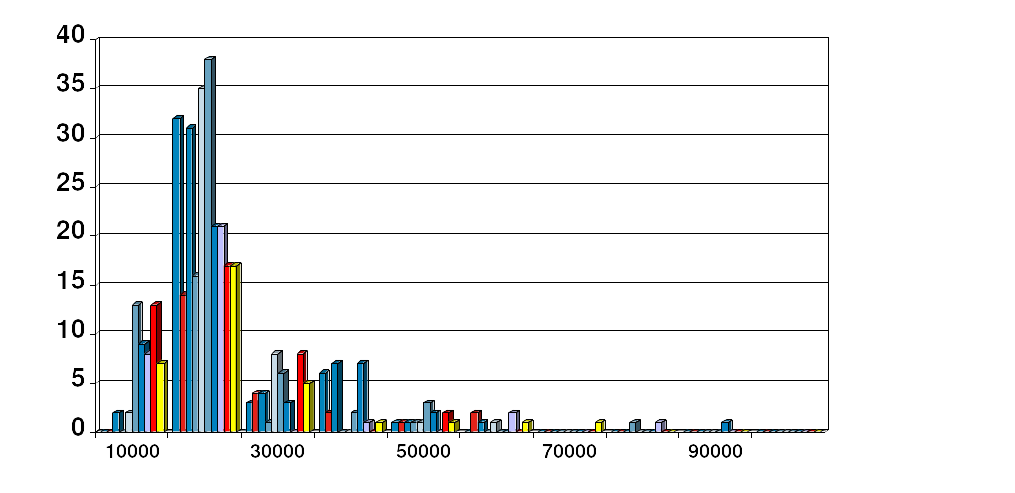
\includegraphics[width=10cm]{img/histogram.png}
\end{frame}

\begin{frame}{Clustering}
	\begin{itemize}
		\item \textbf{Partition data set into clusters based on similarity and 
		store cluster representation (e.g., centroid and diameter) only.}
		\begin{itemize}
			\item Can be very effective if data points are close to each other 
			under a certain norm and choice of space.
			\item Can have hierarchical clustering and be stored in 
			multidimensional index-tree structures.
			\item There are many choices of clustering algorithms.
			\item Cluster analysis will be studied in depth in Chapter 7.
		\end{itemize}
	\end{itemize}
\end{frame}

\begin{frame}{Sampling}
	\begin{itemize}
		\item \textbf{Obtain a small sample $x$ to represent the whole data set 
		$X$.}
		\item \textbf{Allow a mining algorithm to run in complexity \\ that is 
		potentially sub-linear to the size of the data.}
		\item \textbf{Key principle: Choose a 
		{\color{airforceblue}representative} subset of the data.}
		\begin{itemize}
			\item Simple random sampling may have very poor performance in the 
			presence of skew.
			\item Develop adaptive sampling methods, e.g. stratified sampling.
		\end{itemize}
		\item \textbf{Note: Sampling may not reduce database I/Os.}
		\begin{itemize}
			\item One page at a time.
		\end{itemize}
	\end{itemize}
\end{frame}

\begin{frame}{Types of Sampling}
	\begin{itemize}
		\item \textbf{Simple random sampling.}
		\begin{itemize}
			\item There is an equal probability of selecting any particular 
			item.
		\end{itemize}
		\item \textbf{Sampling without repetition.}
		\begin{itemize}
			\item Once an object is selected, it is removed from the population.
		\end{itemize}
		\item \textbf{Sampling with repetition.}
		\begin{itemize}
			\item A selected object is not removed from the population.
		\end{itemize}
		\item \textbf{Stratified sampling:}
		\begin{itemize}
			\item Partition the data set and draw samples from each partition: 
			Proportionally, i.e. approximately the same percentage of the data.
			\item Used in conjunction with skewed data.
		\end{itemize}
	\end{itemize}
\end{frame}

\begin{frame}{Data-cube Aggregation}
	\begin{itemize}
		\item \textbf{The lowest level of a data cube (base cuboid).}
		\begin{itemize}
			\item The aggregated data for an \textbf{individual entity of 
			interest}.
			\item E.g. a customer in a phone-calling data warehouse.
			\item Number of calls per hour, day, or week.
		\end{itemize}
		\item \textbf{Multiple levels of aggregation in data cubes.}
		\begin{itemize}
			\item Further reduce the size of data to deal with.
		\end{itemize}
		\item \textbf{Reference appropriate levels.}
		\begin{itemize}
			\item Use the smallest representation which is enough to solve the 
			task.
		\end{itemize}
		\item \textbf{Queries regarding aggregated information should be 
		answered using the data cube, if possible.}
	\end{itemize}
\end{frame}

\begin{frame}{Data Reduction (III): Data Compression}
	\begin{itemize}
		\item \textbf{String compression.}
		\begin{itemize}
			\item There are extensive theories and well-tuned algorithms.
			\item Typically lossless, but only limited manipulation is possible 
			without expansion.
		\end{itemize}
		\item \textbf{Audio/video compression.}
		\begin{itemize}
			\item Typically lossy compression, with progressive refinement.
			\item Sometimes small fragments of signal can be reconstructed 
			without reconstructing the whole.
		\end{itemize}
		\item \textbf{Time sequence is not audio.}
		\begin{itemize}
			\item Typically short and varies slowly with time.
		\end{itemize}
		\item \textbf{Dimensionality and numerosity reduction may also be 
		considered as forms of data compression.}
	\end{itemize}
\end{frame}